\documentclass{beamer}
\usetheme{metropolis}
\usepackage{graphicx}
\usepackage{tcolorbox}
\usepackage{amsmath}
\usepackage{hyperref}
\DeclareMathOperator\erfc{erfc}
\definecolor{box_background}{RGB}{225,225,225}
\definecolor{box_frame}{RGB}{0,0,0}
\title{Complex analysis of Askaryan radiation: energy and angular reconstruction of ultra-high energy neutrinos}
\author{Jordan C. Hanson and Raymond Hartig}
\institute{Dept. of Physics and Astronomy \\ Whittier College \\ Whittier, CA}

\begin{document}
\titlegraphic{\vspace{6cm}\hspace{6.8cm}
\includegraphics[width=4cm,height=2cm]{WhittierImages.pdf}}  
\maketitle

\begin{frame}{Outline: from mathematical physics to UHE-$\nu$ observations}
\begin{columns}[T]
\begin{column}{0.5\textwidth}
\textbf{\alert{Background}}
\begin{itemize}
\item UHE-$\nu$ flux
\item The Askaryan effect
\item RF UHE-$\nu$ detectors
\end{itemize}
\textbf{\alert{The Askaryan signal}}
\begin{itemize}
\item Analytic radiation model
\item Signal \textit{envelopes}
\item Uncertainty principles
\end{itemize}
\textbf{\alert{Event reconstruction}}
\begin{itemize}
\item \textbf{NuRadioMC}: MC software
\item Mathematics $\leftrightarrow$ signals
\item Initial results
\end{itemize}
\end{column}
\begin{column}{0.5\textwidth}
\begin{figure}
\centering
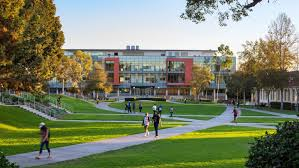
\includegraphics[width=0.9\textwidth]{whittier3.jpeg}
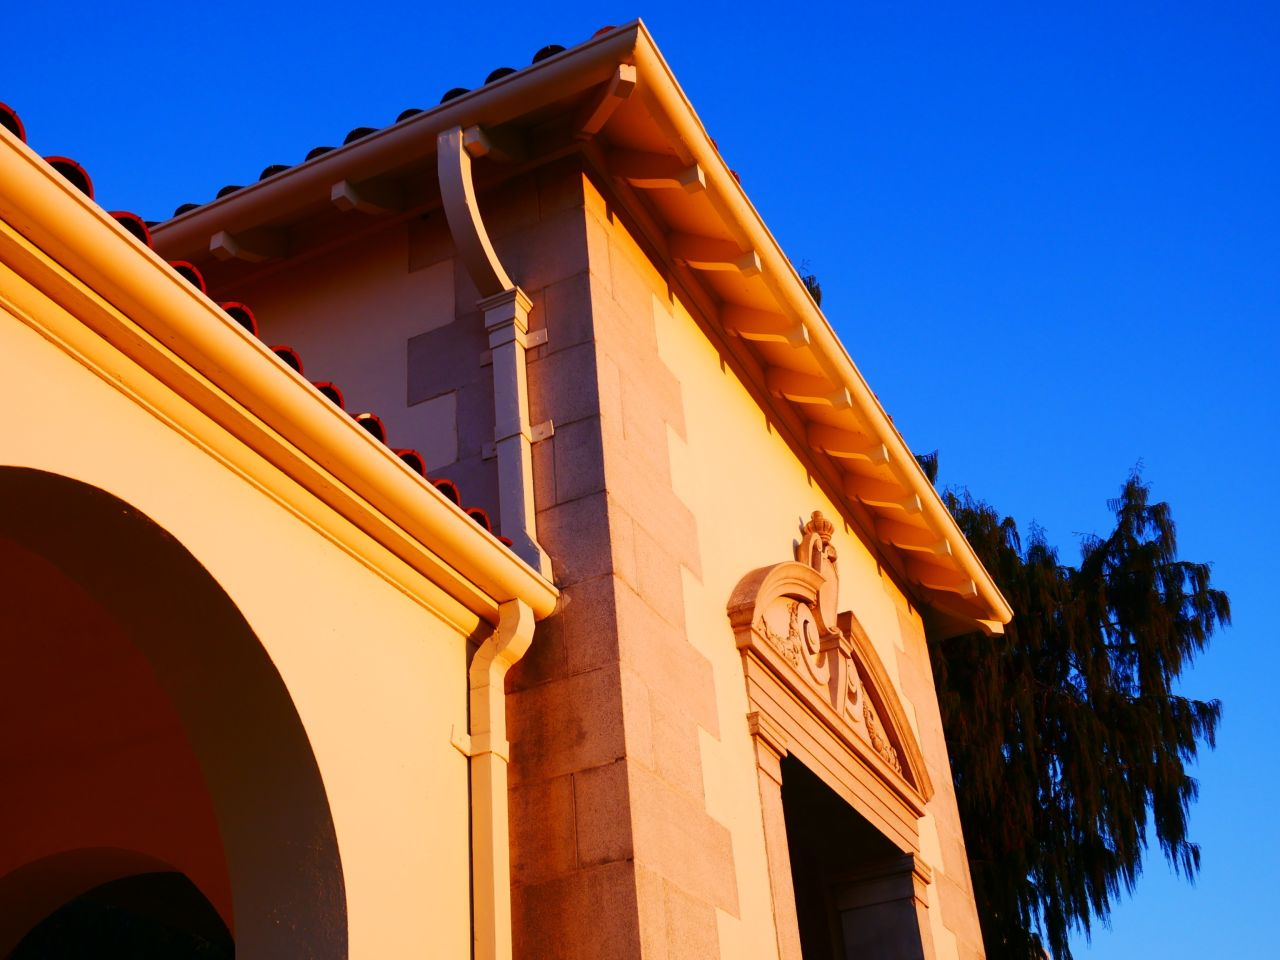
\includegraphics[width=0.9\textwidth]{whittier1.jpeg}
\caption{\small Whittier College.}
\end{figure}
\end{column}
\end{columns}
\end{frame}

\section{Background}

\begin{frame}{Background: in-ice UHE-$\nu$ observations}
\small
\begin{columns}[T]
\begin{column}{0.32\textwidth}
\textbf{\alert{UHE-$\nu$ detection via the Askaryan Effect}}
\begin{itemize}
\item \textbf{E$_{\nu} \geq $10$^{16}$ eV}
\item \textbf{Flux is small}
\item Cascades $\leftrightarrow$ RF
\item Ice is transparent
\item Station arrays
\end{itemize}
\end{column}
\begin{column}{0.68\textwidth}
\begin{figure}
\centering
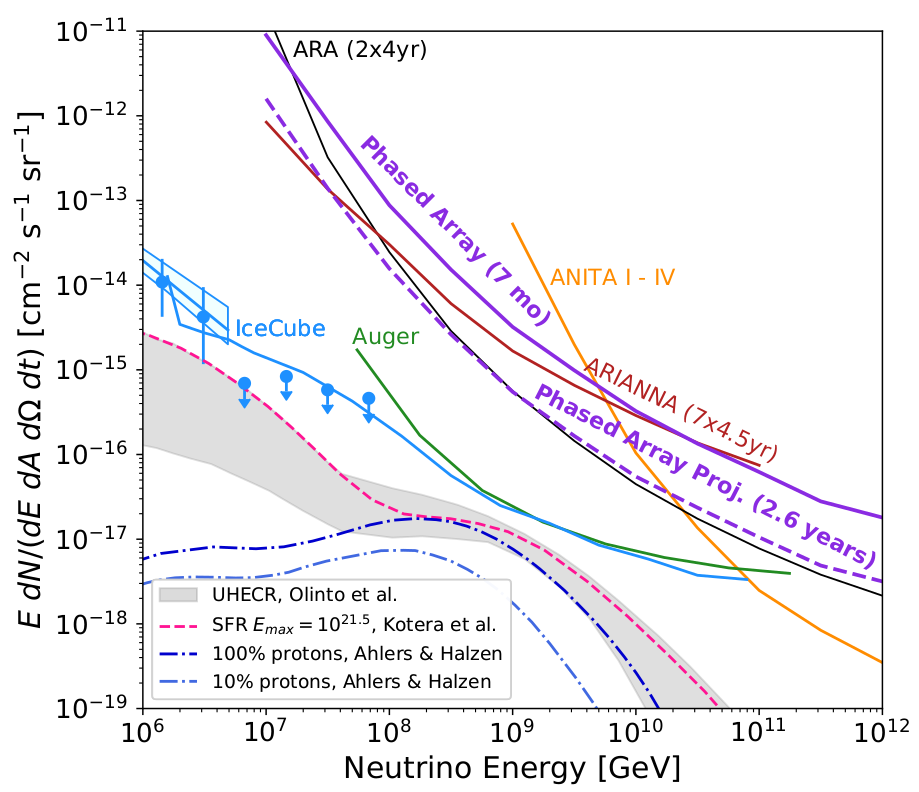
\includegraphics[width=0.9\textwidth]{flux.png}
\caption{\footnotesize UHE-$\nu$ flux predictions and upper limits.}
\end{figure}
\end{column}
\end{columns}
\end{frame}

\begin{frame}{Background: in-ice UHE-$\nu$ observations}
\small
\begin{columns}[T]
\begin{column}{0.32\textwidth}
\textbf{\alert{UHE-$\nu$ detection via the Askaryan Effect}}
\begin{itemize}
\item $E_{\nu} \geq 10^{16}$ eV
\item Flux is small
\item \textbf{Cascades $\leftrightarrow$ RF}
\item Ice is transparent
\item Station arrays
\end{itemize}
\end{column}
\begin{column}{0.68\textwidth}
\begin{figure}
\centering
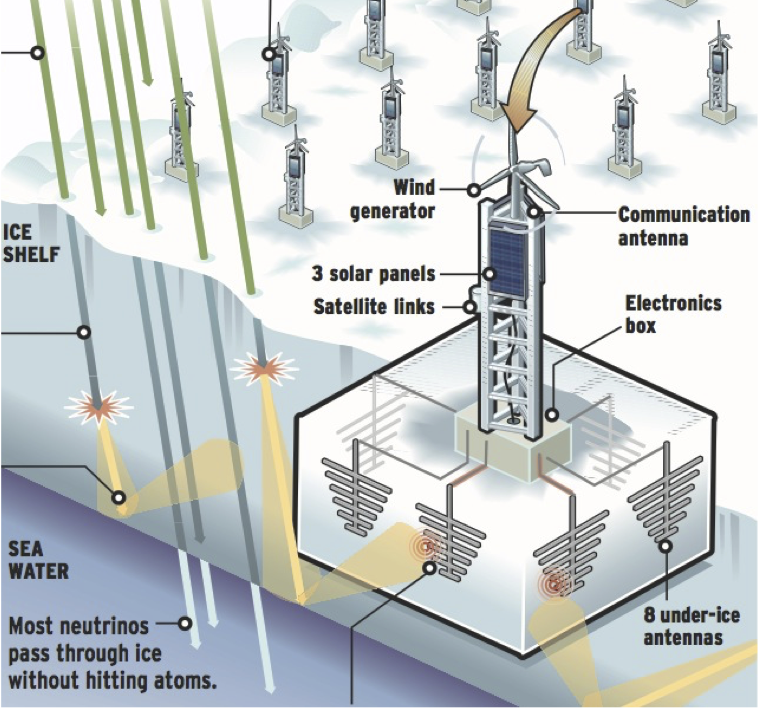
\includegraphics[width=0.5\textwidth]{ARIANNA_principle.png}
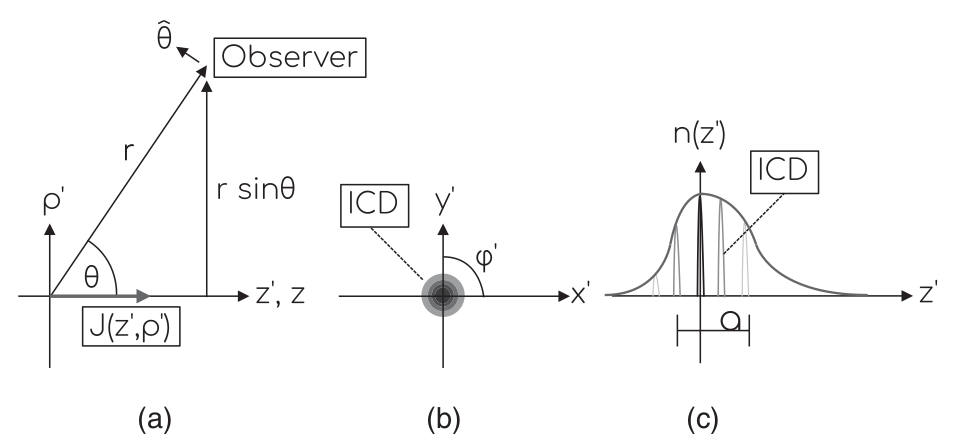
\includegraphics[width=0.9\textwidth]{icd.png}
\caption{\footnotesize The Askaryan effect.}
\end{figure}
\end{column}
\end{columns}
\end{frame}

\begin{frame}{Background: in-ice UHE-$\nu$ observations}
\small
\begin{columns}[T]
\begin{column}{0.32\textwidth}
\textbf{\alert{UHE-$\nu$ detection via the Askaryan Effect}}
\begin{itemize}
\item $E_{\nu} \geq 10^{16}$ eV
\item Flux is small
\item Cascades $\leftrightarrow$ RF
\item \textbf{Ice is transparent}
\item Station arrays
\end{itemize}
\end{column}
\begin{column}{0.68\textwidth}
\begin{figure}
\centering
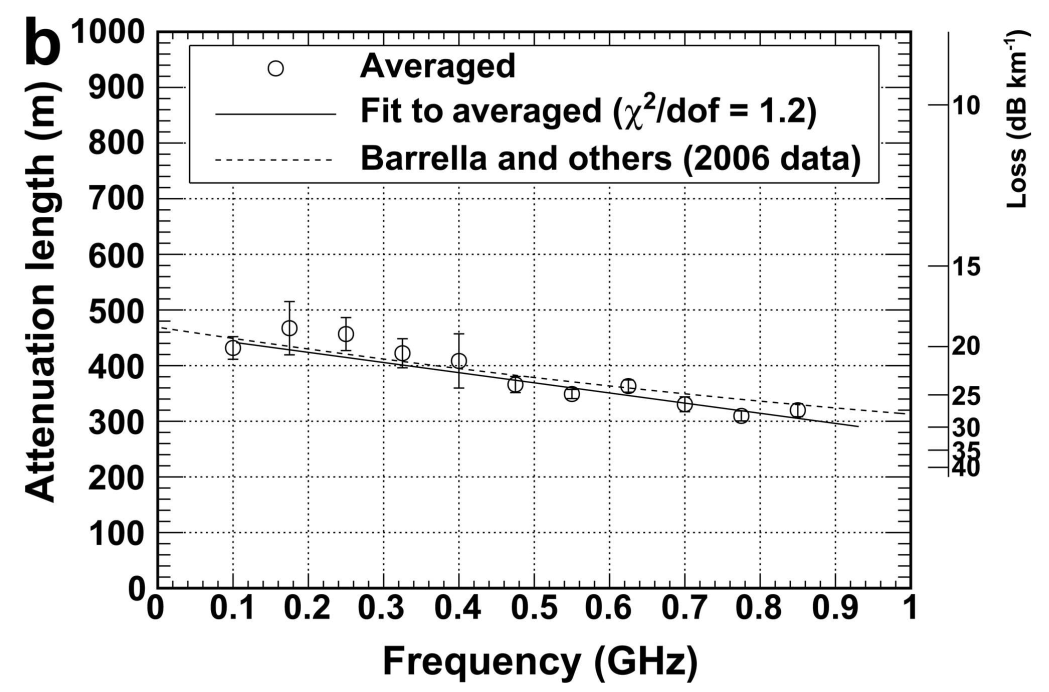
\includegraphics[width=0.6\textwidth]{moores_atten.png}
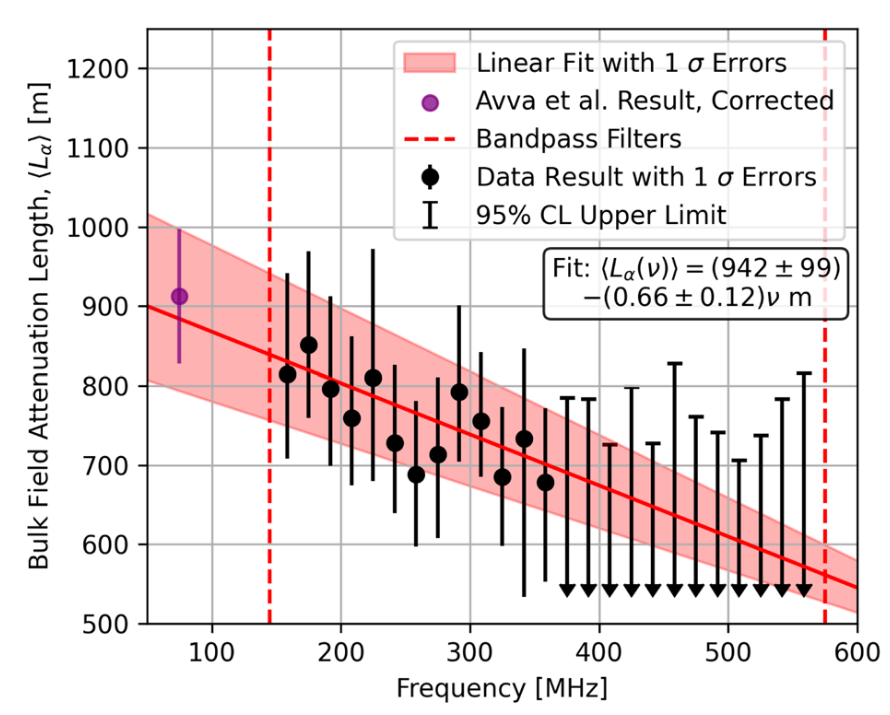
\includegraphics[width=0.6\textwidth]{atten_greenland.png}
\caption{\footnotesize RF attenuation lengths in ice.}
\end{figure}
\end{column}
\end{columns}
\end{frame}

\begin{frame}{Background: in-ice UHE-$\nu$ observations}
\small
\begin{columns}[T]
\begin{column}{0.32\textwidth}
\textbf{\alert{UHE-$\nu$ detection via the Askaryan Effect}}
\begin{itemize}
\item $E_{\nu} \geq 10^{16}$ eV
\item Flux is small
\item Cascades $\leftrightarrow$ RF
\item Ice is transparent
\item \textbf{Station arrays}
\end{itemize}
\end{column}
\begin{column}{0.68\textwidth}
\begin{figure}
\centering
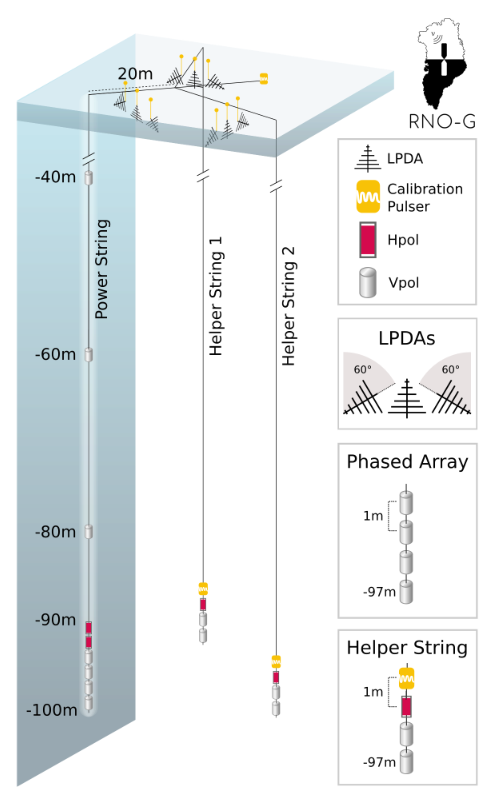
\includegraphics[width=0.35\textwidth]{RNO-G.png} \hspace{0.5cm}
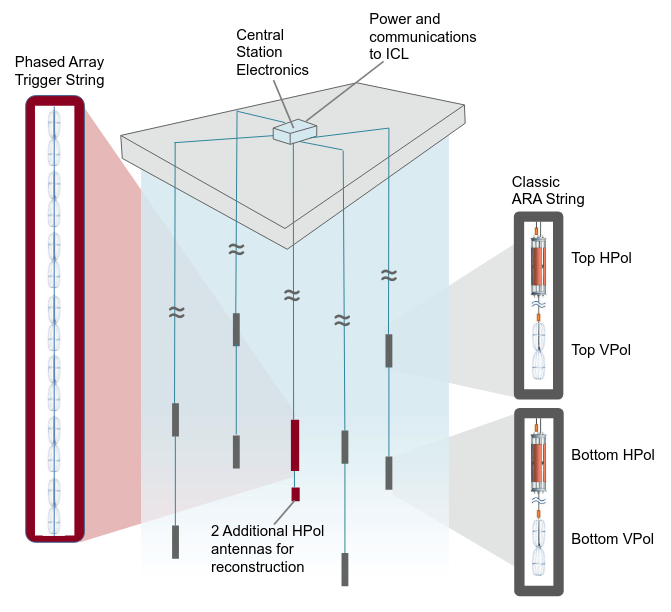
\includegraphics[width=0.55\textwidth]{ARA.png}
\caption{\footnotesize In-ice UHE-$\nu$ detectors. \textbf{Left:} RNO-G (Greenland). \textbf{Right:} ARA (Antarctica).}
\end{figure}
\end{column}
\end{columns}
\end{frame}

\section{The Askaryan Signal}

\begin{frame}{The Askaryan Signal: equation for $\vec{E}$-field}
\begin{tcolorbox}[colback=box_background,colframe=box_frame,title={Askaryan electric field, $\vec{E}(r,t)$, [V m$^{-1}$]}]
\begin{equation}
r \vec{E}(t,\theta) = -\frac{E_0 \omega_0 \sin(\theta)}{8 \pi p} t_r e^{-\frac{t_r^2}{4p} + p \omega_0^2}\erfc(\sqrt{p}\omega_0)
\end{equation}
\end{tcolorbox}
\footnotesize
\begin{columns}[T]
\begin{column}{0.49\textwidth}
\textbf{Geometric parameters}
\begin{table}
\centering
\begin{tabular}{c|c}
$r$ & vertex distance [m] \\
$E_0$ & E-field amplitude [V GHz$^{-2}$] \\
$t_r$ & Retarded time [ns]\footnote{Definition: $t_{\rm r} = t_{\rm ref} - nR/c$.} \\
$\theta$ & Observation angle [rad] \\
$p$ & $\sigma_t = \sqrt{2p}$ (Eq. \ref{eq:p}) [ns$^2$]
\end{tabular}
\end{table}
\end{column}
\begin{column}{0.49\textwidth}
\textbf{Particle physics parameters}
\begin{table}
\centering
\begin{tabular}{c|c}
$\omega_0$ & Form-factor frequency [GHz] \\
$\theta_{\rm C}$ & Cherenkov angle [rad] \\
$p$ & $\sigma_t = \sqrt{2p}$ (Eq. \ref{eq:p}) [ns$^2$] \\
$a$ & Cascade length (Eq. \ref{eq:p}) [m]
\end{tabular}
\end{table}
\begin{align}
p =& \frac{1}{2}\left(\frac{a}{c}\right)^2 \left(\cos\theta - \cos\theta_C\right)^2 \label{eq:p} \\
\sqrt{2p} \approx & ~(a/c)|\theta - \theta_{\rm C}|\sin\theta_{\rm C} \\
\sigma_t =& \sqrt{2p} \propto ~ a\Delta\theta
\end{align}
\end{column}
\end{columns}
\end{frame}

\begin{frame}{The Askaryan Signal: $\vec{E}$-field time-dependence, analytic signal}
\begin{tcolorbox}[colback=box_background,colframe=box_frame,title={Askaryan electric field, $\vec{E}(r,t)$, [V m$^{-1}$], time-dependence}]
\begin{equation}
s(t) = \vec{E}(t,\theta) = -E_0 t e^{-\frac{1}{2}\left(\frac{t}{\sigma_t}\right)^2}
\end{equation}
\end{tcolorbox}
\begin{tcolorbox}[colback=box_background,colframe=box_frame,title={Askaryan electric field \textit{analytic signal}}]
\begin{equation}
s_a(t) = -E_0 \left(t e^{-\frac{1}{2}\left(t/\sigma_t\right)^2} - \frac{2 j\sigma_t}{\sqrt{2\pi}} \frac{dD(x)}{dx}\right)
\end{equation}
\end{tcolorbox}
\footnotesize
\begin{columns}[T]
\begin{column}{0.49\textwidth}
\textbf{The signal envelope}
\begin{itemize}
\item $s_a(t) = s(t) + j ~ \widehat{s}(t)$
\item $\widehat{s}(t)$, Hilbert transform
\item $|s_a(t)|$, signal \textit{envelope}
\end{itemize}
\end{column}
\begin{column}{0.49\textwidth}
\textbf{Special functions and variables}
\begin{itemize}
\item $D(x)$, Dawson function
\item $x = t/(\sqrt{2}\sigma_t)$, normalized time
\end{itemize}
\end{column}
\end{columns}
\end{frame}

\begin{frame}{The Askaryan Signal: detected signals}
\begin{tcolorbox}[colback=box_background,colframe=box_frame,title={Common response function for RF channels $r(t)$, [m ns$^{-1}$]}]
\begin{equation}
r(t) = R_0 \cos(2\pi f_0 t) e^{-\gamma t}
\end{equation}
\end{tcolorbox}
\begin{tcolorbox}[colback=box_background,colframe=box_frame,title={Common analytic signal for RF channels $r_a(t)$, [m ns$^{-1}$]}]
\begin{equation}
r_a(t) = R_0 e^{2\pi j f_0 t-\gamma t}
\end{equation}
\end{tcolorbox}
\footnotesize
\begin{columns}[T]
\begin{column}{0.49\textwidth}
\textbf{The signal envelope}
\begin{itemize}
\item $r_a(t) = r(t) + j ~ \widehat{r}(t)$
\item $\widehat{r}(t)$, Hilbert transform
\item $|r_a(t)|$, signal \textit{envelope}
\end{itemize}
\end{column}
\begin{column}{0.49\textwidth}
\textbf{RF channels: RLC circuits}
\begin{itemize}
\item $|r_a(t)| = R_0\exp(-\gamma t)$
\item $\gamma$, damping coefficient [GHz]
\item $f_0$, resonance frequency [GHz]
\end{itemize}
\end{column}
\end{columns}
\end{frame}

\begin{frame}{The Askaryan Signal: detected signals}
\begin{tcolorbox}[colback=box_background,colframe=box_frame,title={Detected signals, $r(t) * s(t)$, [V]}]
\begin{equation}
r(t) * s(t) = \int_{-\infty}^{\infty} r(\tau) s(t-\tau) d\tau \rightarrow \int_{0}^{\infty} r(\tau) s(t-\tau) d\tau
\end{equation}
\end{tcolorbox}
\begin{tcolorbox}[colback=box_background,colframe=box_frame,title=Theorem: the envelope of detected signal]
Let $\mathcal{E}_{r * s}(t)$ represent the \textit{envelope} of the convolution of $r(t)$ and $s(t)$.  If $s_a(t)$ and $r_a(t)$ are the analytic signals of $s(t)$ and $r(t)$, respectively, then
\begin{equation}
\mathcal{E}_{r*s}(t) = \frac{1}{2}|r_a(t) * s_a(t)|
\end{equation}
\end{tcolorbox}
\end{frame}

\begin{frame}{The Askaryan Signal: uncertainty principles}
\begin{tcolorbox}[colback=box_background,colframe=box_frame,title={Uncertainty principles within Askaryan field}]
Let $\Delta\theta = \theta - \theta_{\rm C}$.  Let $a$ be the cascade length, $c$ be the speed of light, $\sigma_t$ be the pulse width, and $\sigma_f$ be the width of the Fourier spectrum.
\begin{equation}
a\Delta\theta = \frac{c\sigma_t}{\sin\theta_{\rm C}}
\end{equation}
Further, $s(t)$, and $S(f)$ (the Fourier transform), have widths that satisfy
\begin{equation}
\sigma_t \sigma_f = \frac{1}{2\pi}\left(1+\eta^2\right)^{1/2}
\end{equation}
In the far-field, $\eta \to 0$.
\end{tcolorbox}
\end{frame}

\begin{frame}[fragile]{The Askaryan Signal: scanning $a$ and $\Delta\theta$}
\begin{figure}
\centering
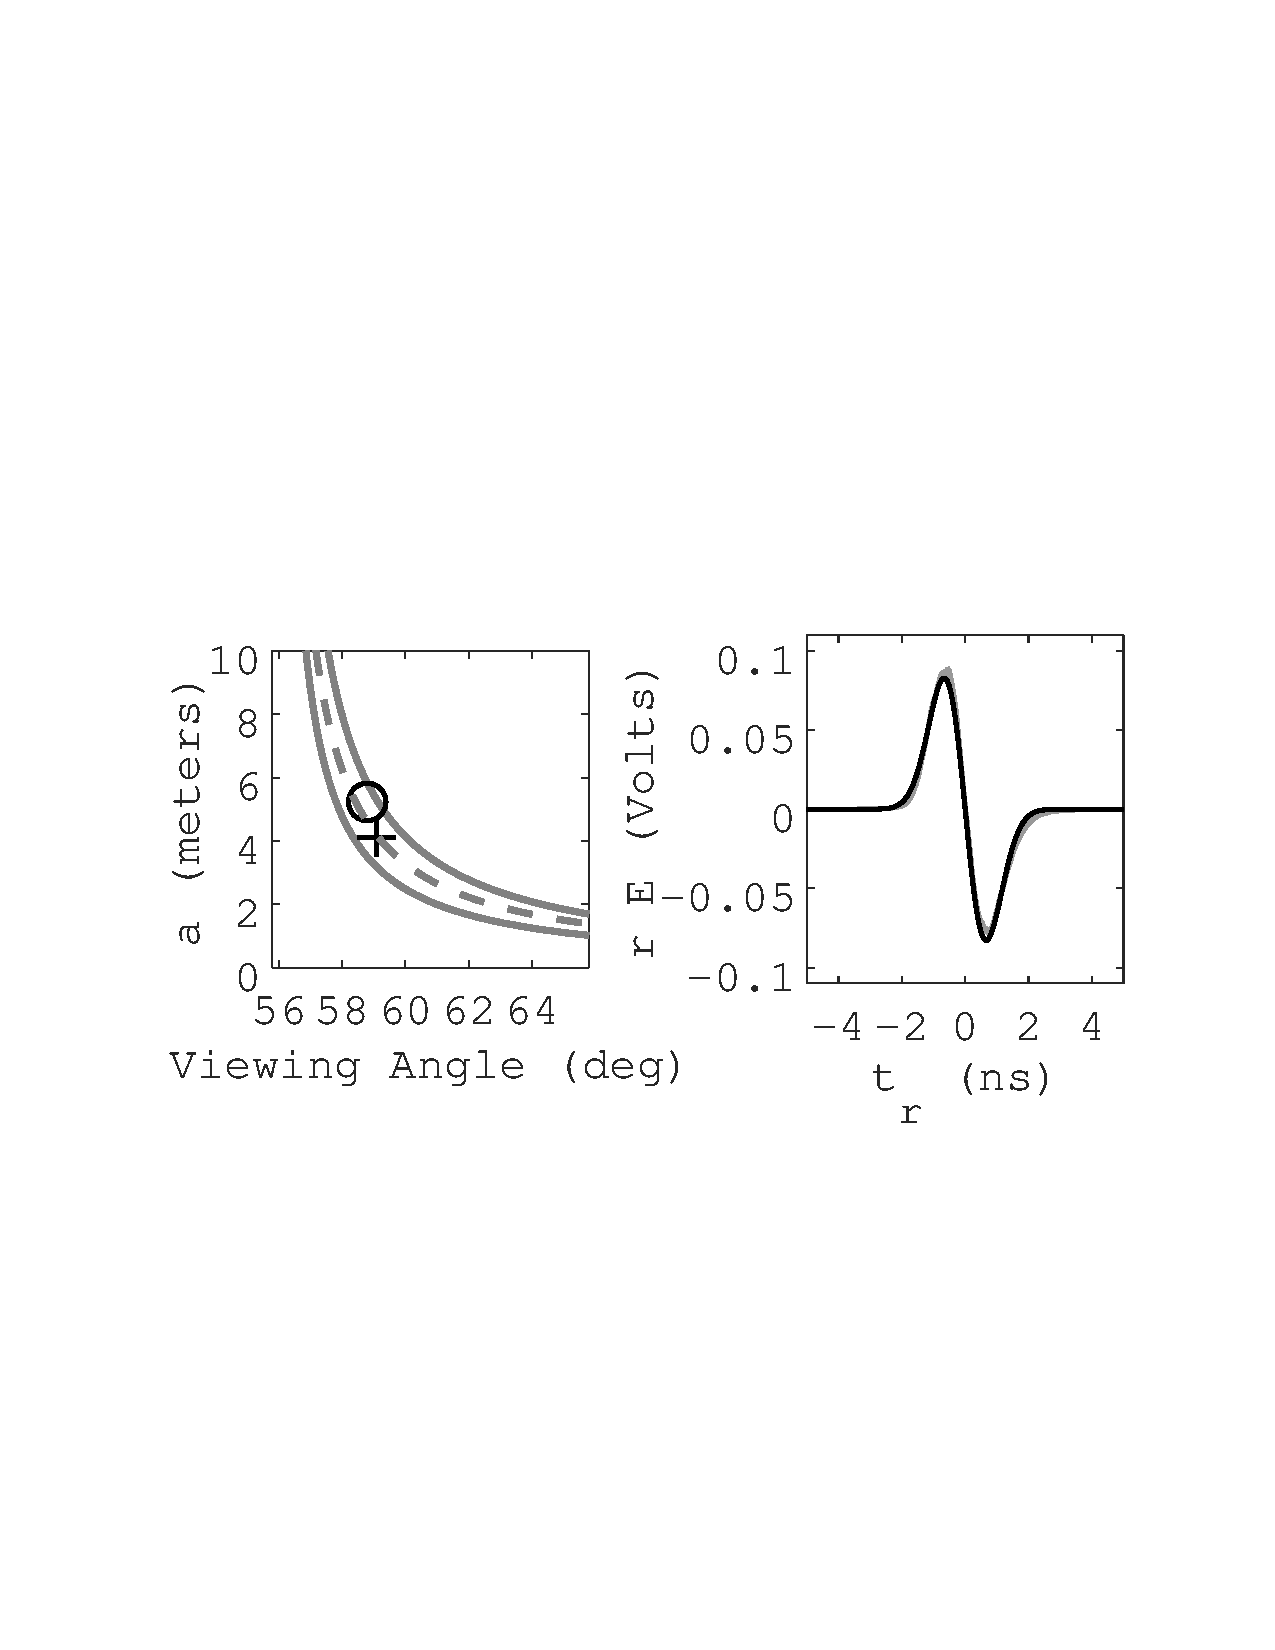
\includegraphics[width=0.75\textwidth,trim=2cm 9cm 2cm 10cm,clip=true]{example_scan.pdf}
\caption{\label{fig:scan} Scanning Askaryan field equation parameters to fit NuRadioMC output.}
\end{figure}
\textbf{Energy reconstruction potential:} $a^2 \propto \ln(E_{\rm C}/E_{\rm crit})$
\end{frame}

\section{Conclusion}

\begin{frame}{Unit 1.1 Outline}
Unit 1.1 covered:

\end{frame}

\end{document}
